\documentclass[a4paper,12pt]{article}

% Pakiety do różnych funkcji
\usepackage[a4paper,left=2cm,right=2cm,top=\dimexpr15mm+2.5\baselineskip,bottom=3cm]{geometry}
\usepackage{amsmath, amssymb} % For mathematical symbols
\usepackage{multicol}         % Tworzenie wielokolumnowego tekstu
\usepackage{array}            % Ulepszone tabele
\usepackage{graphicx}         % Dodawanie obrazków
\usepackage{float}
\usepackage{color}            % Kolorowanie tekstu
\usepackage{hyperref}         % Hiperłącza w dokumencie
\usepackage{listings}         % Wstawianie kodu źródłowego
\usepackage[utf8]{inputenc}   % Obsługuje kodowanie UTF-8
\usepackage[T1]{fontenc}      % Obsługuje polskie znaki i inne znaki spoza ASCII
\usepackage[polish]{babel}    % Ustawienia języka polskiego
\usepackage{fancyhdr}         % For header and footer
\usepackage{lastpage}         % For total number of pages
\usepackage{lmodern}          % Better font rendering
\usepackage{titlesec}         % For adjusting title spacing
\usepackage{wrapfig}
\usepackage{centernot}
\usepackage{enumitem}
\usepackage[dvipsnames]{xcolor} % Więcej kolorków dla komendy \color
\usepackage{needspace}

% Line spacing adjustments
\linespread{0.8}  % Makes lines less tight
% Header & Footer Setup
\pagestyle{fancy}
\fancyhf{}
\fancyhfoffset[L]{1mm} % left extra length
\fancyhfoffset[R]{1mm} % right extra length
\fancyhead[L]{\textbf{\huge Title}}    % Title on the left (bigger)
\fancyhead[C]{\text{Kacper Poneta \\ Kacper Orszulak \\ Natalia Ignatowicz}} % Author in the middle (bigger)
\fancyhead[R]{\text{\today}}         % Date on the right (bigger)
\fancyfoot[R]{\thepage/\pageref{LastPage}} % Page number in format current/total

% Build info or date on the right of the header
\makeatletter
\@ifundefined{buildHeader}{
  \newcommand{\buildHeader}{\today}
}{}
\makeatother
\fancyhead[R]{\buildHeader}

% Add vertical space before the header line (custom space before the rule)
\renewcommand{\headrulewidth}{0.4pt}    % Header line thickness
\renewcommand{\headrule}{\vspace{10pt}\hrule}  % Add 10pt space above the header line

% Footer setup and add space before the footer line
\renewcommand{\footrulewidth}{0.4pt}    % Footer line thickness
\setlength{\headheight}{50pt}

% Break the page if new section would start near the end of the page
\pretocmd{\section}{%
  \needspace{60ex}%
}{}{}


\fancyhead[L]{\text\substack{\textbf{Projekt sklepu \\ internetowego} \\ \textit{Cloth Craft}}}    % Title on the left (bigger)

% Document Body
\begin{document}

\section*{\textit{Cloth Craft}}

Sklep całkowicie internetowy z ubraniami.

\begin{figure}[h] % 'h' means here; you can also use 't' for top, 'b' for bottom, etc.
    \centering % Center the figure
    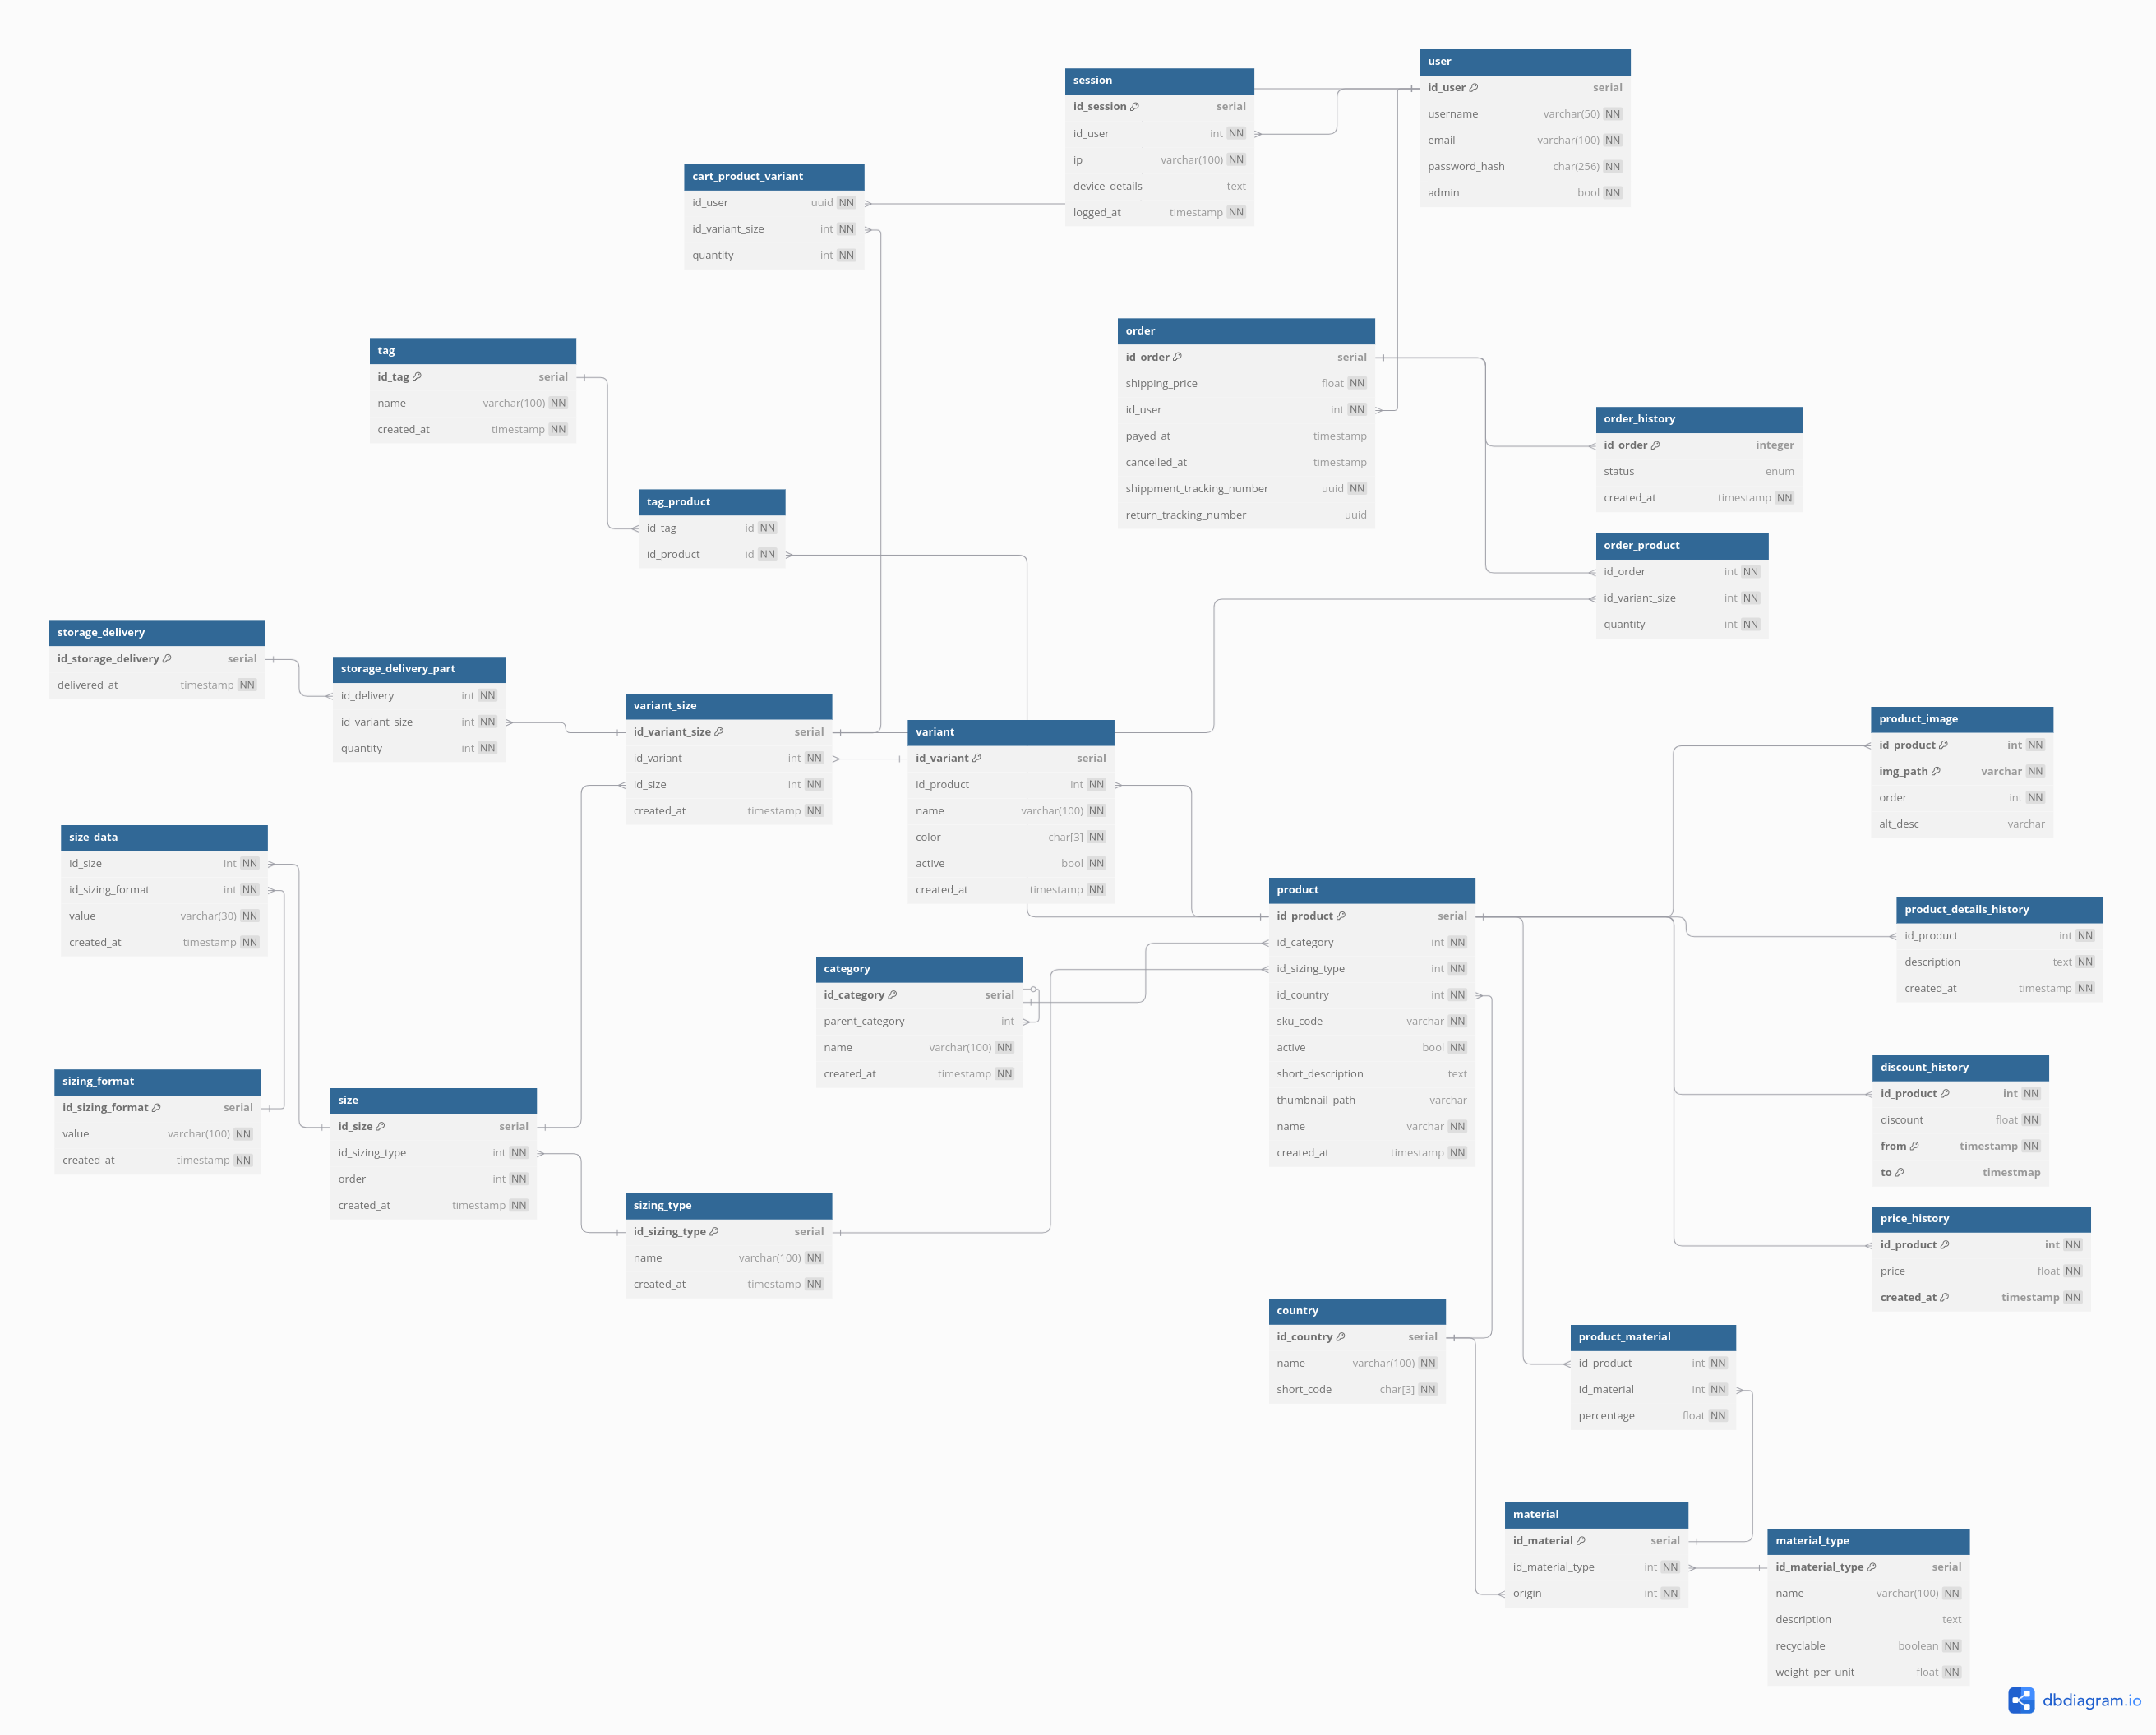
\includegraphics[width=1.0\textwidth]{diagram.png} % Adjust the width as needed
    \caption{Diagram bazy danych.} % Optional caption
    \label{fig:example} % Optional label for referencing
\end{figure}

\section*{Szczegóły niektórych tabel}

\subsection*{Zmienialność tabel i historia zmian}
Domyślnie dane we wszystkich tabelach są niezmienialne po wstawieniu, a encje nie mogą być usuwane. Dzięki temu nie ma ryzyka, że klient kupuje produkt, a potem, gdy chce się odwołać do jego opisu, opis jest nieaktualny. Encje tylko niektórych tabel mogą być zmieniane. Wiele obiektów ma możliwość tworzenia historii, a więc nie ma potrzeby wprowadzania zmian.

Tabele, których encje mogą być modyfikowane i usuwane: Przede wszystkim użytkownicy i sesje.

Dodatkowo pozwalamy na usuwanie i zmianę tagów. Jest to rodzaj informacji, który jedynie pomaga w filtrowaniu.

Aby nie pozwolić na usuwanie i zmiany, po prostu nie dajemy takiej możliwości w API. Nie ograniczamy tego na poziomie bazy danych.

Dodatkowo pozwalamy na ustawienie \texttt{active} dla produktu i wariantu jako fałsz/prawdę. Przydaje się to w sytuacji np., kiedy dany produkt nie będzie już dłużej dostępny, ale chcemy by klienci, którzy kupili produkt nadal mieli dostęp do informacji o produkcie. Podobnie dany wariant może zostać wycofany.

\subsection*{Logika reprezentacji produktów i wariantów}
Każde ubranie może występować w wielu wariantach i rozmiarach. Wariant jest charakteryzowany przede wszystkim przez kolor i ewentualne inne cechy szczególne. Każdy wariant jest dostępny w potencjalnie wielu rozmiarach. Zależnie od produktu typ tego rozmiaru (\texttt{sizing\_type}) może być inny: rozmiar butów nie jest porównywalny np. z rozmiarem koszulek, czy spodni. Ponadto każdy rozmiar (\texttt{size}) może być wyrażany w różny sposób (np. za pomocą różnych jednostek). Różne reprezentacje jednego rozmiaru obsługuje tabela \texttt{size\_data}, która ponadto przechowuje informacje o formacie (\texttt{sizing\_format}).

\subsection*{\texttt{product\_details\_history}}
\texttt{description} będzie przechowywany jako Markdown. Będziemy go renderować za pomocą biblioteki JavaScript.

\subsection*{\texttt{cart\_product\_variant}}
Zawartość każdego koszyka nieużywanego odpowiednio długo jest usuwany za pośrednictwem cron job. Dodanie produktu do koszyka nie blokuje innych użytkowników przed dodaniem go również. Kupienie zawartości koszyka tworzy zamówienie. Przy tworzeniu zamówienia zmiejsza się dostępność produktów.

\subsection*{\texttt{order\_history}}
Możliwe statusy:
\texttt{
    paid, pending, shipped, delivered, cancelled,
    return\_requested, return\_rejected, return\_pending,
    return\_shipped, return\_delivered
}

\section*{Aspekty logiki aplikacji}
\subsection*{Płatności}
Użytkownik podaje dane karty płatniczej. Nie są one weryfikowane, a płatność zawsze jest akceptowana.

\subsection*{Koszty dostawy}
Domyślnie koszt dostawy to zawsze ustalona z góry wartość. Gdy wartość zamówienia jest odpowiednio wysoka, dostawa staje się darmowa.

\subsection*{Adresy dostawy}
Zakładamy, że firma kurierska przechowuje informacje o adresie dostawy podane podczas składania zamówienia. Każde zamówienie posiada \texttt{shippment\_tracking\_number}, które miało by służyć do łączenia się z API firmy kurierskiej. Oczywiście nie implementujemy komunikacji z żadną firmą kurierską.

\section*{Indeksy}
\begin{itemize}
    \item Nazwy
        \begin{itemize}
            \item Produktów
            \item Tagów
            \item Kategorii
            \item Itd.
        \end{itemize}
    \item Klucze obce
        \begin{itemize}
            \item W celu optymalizacji krytycznych zapytań.
                    \begin{itemize}
                        \item Np. \texttt{variant.product\_id} dla wyświetlania wszystkich wariantów wybranego produktu.
                    \end{itemize}
        \end{itemize}
\end{itemize}

Ponadto indeks częściowy tylko na aktywnych produktach itd..

\section*{Widoki}
Wstępne pomysły na widoki:
\begin{itemize}
    \item Strona główna: przykładowe produkty wraz z kategoriami i tagami.
    \item Statystyki wszystkich koszyków.
    \item Dostępne produkty wraz z wariantami i rozmiarami.
    \item Zniżki o kończącej się dacie ważności.
\end{itemize}

\section*{Funkcje}
\begin{itemize}
    \item Sprawdź zawartość koszyka wraz z dostępnością dodanych produktów.
    \item Liczenie sumarycznej ilości wariantów na podstawie historii dostaw do magazynu.
    \item Liczenie całkowitego kosztu zamówienia na podstawie czasu złożenia zamówienia i historii cen.
    \item Wyświetl listę nadrzędnych kategorii.
    \item Generowanie wyników wyszukiwania na podstawie filtrów.
\end{itemize}

\section*{Wyzwalacze}
\subsection*{Spójność typów rozmiarów}
Z jednej strony produkt definiuje typ rozmiaru, który go charakteryzuje, ale każdy rozmiar też jest określonego typu. Niezbędna będzie reguła, która będzie weryfikować przed dodaniem rozmiaru konkretnemu wariantowi produktu, czy typ tego rozmiaru się zgadza.

\subsection*{Weryfikacja poprawności składu materiału}
Wyzwalacz na sumę procentu udziału materiałów w produkcie (\le 100\%).

\section*{Dodatkowe funkcjonalności}
\begin{itemize}
    \item Dokonać (prostej) analizy zakupów i np. dla danego klienta wyznaczać produkt, który opłaca się mu polecić (kupował do tej pory podobne rzeczy).
\end{itemize}

\end{document}

